\section{Basic Optimization Concepts}
The fundamental concepts necessary for the mathematical formulation and solution of optimization problems will be examined in detail in this section. These concepts form the foundation for understanding more complex optimization problems.

\subsection{Objective Function and Constraint Functions}

In the mathematical modeling of optimization problems, there are two fundamental components: the objective function and constraint functions.

\subsubsection{Objective Function}
The objective function mathematically expresses the performance criterion to be optimized. This function can be:
\begin{itemize}
    \item Minimized (e.g., cost, weight, energy consumption)
    \item Maximized (e.g., efficiency, strength, stiffness)
\end{itemize}

\begin{figure}[H]
    \centering
    \includegraphics[width=1\textwidth]{weeks_new/imgs/objective_function.png}
    \caption{Objective Function}
    \label{fig:multi_mod}
\end{figure}

\sidenote{Any maximization problem can be converted to a minimization problem by taking the negative of the objective function: \[ \max f(x) = -\min(-f(x)) \]}

\subsubsection{Constraint Functions}
Constraint functions mathematically express the conditions that the design must satisfy:
\begin{itemize}
    \item Equality constraints: $h_j(x) = 0$
    \item Inequality constraints: $g_i(x) \leq 0$
    \item Boundary constraints: $x_L \leq x \leq x_U$ \sidenote{With few exceptions, structural optimization problems are generally expressed with inequality constraints. Depending on the problem, boundary constraints may also be used. However, when a statically indeterminate structure is subject to optimization, this constraint can also lead to missing the global optimum.
    
    In fact, one of the aspects that makes structural optimization problems worth examining from an optimization perspective is that this statical indeterminacy significantly increases the unpredictability of many structural optimization problems.}
\end{itemize}

\textbf{Equality constraints: $h_j(x) = 0$}
Equality constraints express situations where design variables must take exactly specific values. These types of constraints mathematically define conditions where certain parameters must be precisely satisfied within the optimization problem. For example, a structure's total weight being equal to a specific value or mass balance in a chemical reaction can be expressed with equality constraints. Equality constraints generally keep the optimization space in a narrower area, significantly reducing the number of possible solutions.

\begin{figure}[H]
    \centering
    \includegraphics[width=1\textwidth]{weeks_new/imgs/equality_constraints.png}
    \caption{Equality Constraints}
    \label{fig:}
\end{figure}

\textbf{Inequality constraints: $g_i(x) \leq 0$}
Inequality constraints express situations where design variables must not exceed certain limits. These types of constraints are used to define limitations such as the maximum stress a structure can withstand, a system's maximum energy consumption, or a material's minimum safety factor. Inequality constraints are critical for ensuring that the design is physically realizable and safe. Additionally, inequality constraints define the feasible solution area, ensuring that the optimization algorithm searches only within the valid design space.

\begin{figure}[H]
    \centering
    \includegraphics[width=1\textwidth]{weeks_new/imgs/inequality_constraints.png}
    \caption{Inequality Constraints}
    \label{fig:}
\end{figure}

\textbf{Boundary constraints: $x_L \leq x \leq x_U$}
Boundary constraints determine the minimum and maximum values that each design variable can take. These constraints reflect the physical limits of design variables, manufacturability conditions, or ranges determined by standards. For example, situations where a beam's thickness cannot be less than a certain value due to manufacturing constraints or cannot exceed a certain maximum value due to installation requirements are expressed with boundary constraints. Boundary constraints narrow the optimization algorithm's search space, increasing computational efficiency and ensuring the elimination of physically meaningless solutions.

\begin{figure}[H]
    \centering
    \includegraphics[width=1\textwidth]{weeks_new/imgs/boundary_constraints.png}
    \caption{Boundary Constraints}
    \label{fig:}
\end{figure}

\begin{marginfigure}
\centering
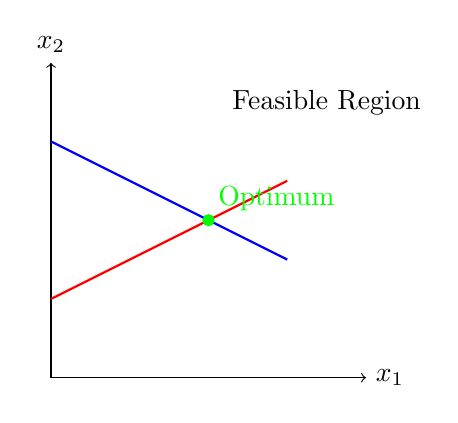
\begin{tikzpicture}
\draw[->] (0,0) -- (4,0) node[right] {$x_1$};
\draw[->] (0,0) -- (0,4) node[above] {$x_2$};
\draw[blue,thick] plot[smooth] coordinates {(0,3) (1,2.5) (2,2) (3,1.5)};
\draw[red,thick] plot[smooth] coordinates {(0,1) (1,1.5) (2,2) (3,2.5)};
\filldraw[green] (2,2) circle (2pt) node[above right] {Optimum};
\node at (3.5,3.5) {Feasible Region};
\end{tikzpicture}
\caption{Feasible solution region formed by the intersection of two constraints}
\label{fig:feasible_region}
\end{marginfigure}

\subsection{Decision Variables and Solution Space}

\subsubsection{Decision Variables}
Decision variables are parameters whose values need to be determined during the optimization process:
\begin{itemize}
    \item Continuous variables (e.g., dimensions, thicknesses)
    \item Discrete variables (e.g., number of elements)
    \item Binary variables (0-1 decisions)
\end{itemize}

\begin{tcolorbox}[title=Decision Variables in Structural Design]
In a steel frame optimization:
\begin{itemize}
    \item \textbf{Continuous:} Section dimensions
    \item \textbf{Discrete:} Number of stories
    \item \textbf{Binary:} Existence/non-existence of elements
\end{itemize}
\end{tcolorbox}

\subsubsection{Solution Space}
The solution space is the space formed by all possible combinations of decision variables\sidenote{The dimension of the solution space is determined by the number of decision variables. In high-dimensional problems, the "curse of dimensionality" problem arises.}:
\begin{itemize}
    \item \textbf{Feasible Solution Region:} Set of points satisfying all constraints
    \item \textbf{Infeasible Region:} Points violating at least one constraint
\end{itemize}

\subsection{Global and Local Minimum/Maximum Concepts}

\subsubsection{Local Optimum}
A point is a local optimum if it has the best value within a certain neighborhood:
\begin{equation}
x^* \text{ local minimum } \Leftrightarrow f(x^*) \leq f(x), \forall x \in N(x^*)
\end{equation}

\subsubsection{Global Optimum}
The point with the best value in the entire solution space is the global optimum:
\begin{equation}
x^* \text{ global minimum } \Leftrightarrow f(x^*) \leq f(x), \forall x \in S
\end{equation}

\begin{figure}
\centering
\begin{tikzpicture}
\draw[->] (0,0) -- (7,0) node[right] {$x$};
\draw[->] (0,-1) -- (0,4) node[above] {$f(x)$};
\draw[scale=1,domain=0:7,smooth,variable=\x,blue] plot ({\x},{1 + sin(3*\x r)+sin(\x r)+sin(0.5*\x r)});
\filldraw[gray] (1.526,1.699) circle (2pt) node[below] {Local};
\filldraw[gray] (3.774,0.412) circle (2pt) node[below] {Local};
\filldraw[black] (5.719,-0.249) circle (2pt) node[below] {Global};
\end{tikzpicture}
\caption{Local and global minimum points of a function}
\label{fig:local_global}
\end{figure}

\subsection{Physical and Mathematical Modeling}

\subsubsection{Physical Modeling}
Modeling real-world problems based on physical principles\sidenote{A good mathematical model should reflect physical reality with sufficient accuracy while avoiding unnecessary complexity. While this is not essentially the main topic of optimization, it is quite important from a structural optimization perspective.}:
\begin{itemize}
    \item Force equilibrium
    \item Energy conservation
    \item Material behavior
    \item Geometric relationships
\end{itemize}

\subsubsection{Mathematical Modeling}
Transforming the physical model into mathematical formulation:
\begin{itemize}
    \item Differential equations
    \item Algebraic equations
    \item Matrix formulations
    \item Finite element models
\end{itemize}

\subsection{Differentiability and Continuity}

\subsubsection{Continuity}
A function being continuous means that small input changes do not cause sudden jumps in the output. Mathematically:
\begin{equation}
\lim_{x \to x_0} f(x) = f(x_0)
\end{equation}

\begin{tcolorbox}[title=Relationship Between Continuity and Optimization]
Continuity is an important property in optimization problems because:
\begin{itemize}
    \item For continuous functions, there must be a minimum and maximum value in a closed and bounded interval (Weierstrass theorem).
    \item Optimization of non-continuous functions is more difficult because sudden jumps can prevent algorithms from progressing in the right direction.
    \item Most physical behaviors in real engineering problems are modeled with continuous functions (e.g., deformation of a beam under load).
\end{itemize}
\end{tcolorbox}

\subsubsection{Differentiability}
The existence of a function's derivative means that the function's behavior can be approximately expressed with a tangent line at every point. Mathematically:
\begin{equation}
f'(x_0) = \lim_{h \to 0} \frac{f(x_0 + h) - f(x_0)}{h}
\end{equation}

\begin{tcolorbox}[title=Relationship Between Differentiability and Optimization]
Differentiability plays a critical role in the optimization process:
\begin{itemize}
    \item \textbf{Gradient Information:} The derivative gives the direction of fastest increase/decrease of the function, so optimization algorithms know where to go.
    \item \textbf{Critical Points:} Points where the function's derivative is zero (critical points) are potential optimum points.
    \item \textbf{Second Derivative:} The second derivative helps determine whether a critical point is a minimum, maximum, or saddle point.
\end{itemize}
\end{tcolorbox}

\begin{marginfigure}
    \centering
    \begin{tikzpicture}
    \draw[->] (0,0) -- (6,0) node[right] {$x$};
    \draw[->] (0,0) -- (0,4) node[above] {$f(x)$};
    
    % Function
    \draw[blue, thick, domain=0:6, smooth, variable=\x] plot ({\x}, {0.1*\x*\x*\x - 0.9*\x*\x + 2*\x + 0.5});
    
    \end{tikzpicture}
    \caption{Differentiable Function and Gradient}
    \label{fig:differentiability}
\end{marginfigure}

\begin{marginfigure}
    \centering
    \begin{tikzpicture}
    \draw[->] (0,0) -- (6,0) node[right] {$x$};
    \draw[->] (0,0) -- (0,4) node[above] {$f(x)$};
    
    % Non-differentiable function (absolute value)
    \draw[blue, thick, domain=0:3, smooth, variable=\x] plot ({\x}, {3-\x});
    \draw[blue, thick, domain=3:6, smooth, variable=\x] plot ({\x}, {\x-3});
    
    % Critical point (corner)
    \filldraw[red] (3,0) circle (2pt) node[below right] {$f'(x)$ undefined};
    
    \end{tikzpicture}
    \caption{Non-differentiable Function (Absolute Value Function)}
    \label{fig:non_differentiable}
\end{marginfigure}

\begin{tcolorbox}[title=Real-Life Example: Mountain Climbing]
Imagine you're climbing a mountain and your goal is to reach the summit. If it's a foggy day and your visibility is very limited, how should you proceed?

\begin{itemize}
    \item \textbf{Gradient (Derivative) Information:} At each step, you can feel the slope of the ground with your feet and choose the steepest uphill direction (negative gradient).
    \item \textbf{Non-differentiable Points:} If there's a steep cliff (point where derivative is undefined) in your path, you can't proceed directly and need to find a different route.
    \item \textbf{Local Peak vs. Summit:} During your climb, you might reach a small peak (local maximum), but the real summit (global maximum) might be elsewhere.
\end{itemize}

This analogy is very similar to how gradient-based optimization algorithms work.
\end{tcolorbox}

\begin{tcolorbox}[title=Optimization Methods Based on Differentiability]
\begin{itemize}
    \item \textbf{Gradient-Based Methods for Differentiable Functions:}
    \begin{itemize}
        \item \textbf{Gradient Descent:} Proceeds in the direction of fastest decrease of the function.
        \item \textbf{Newton's Method:} Uses second derivative information to achieve faster convergence.
        \item \textbf{Quasi-Newton:} Approximates the second derivative (BFGS, L-BFGS, etc.).
    \end{itemize}
    
    \item \textbf{Gradient-Free Methods for Non-differentiable Functions:}
    \begin{itemize}
        \item \textbf{Simplex Search:} Determines the best direction by comparing function values (Nelder-Mead method).
        \item \textbf{Genetic Algorithms:} Explores the solution space by mimicking evolutionary processes.
        \item \textbf{Particle Swarm Optimization:} Approaches the solution by mimicking group behavior.
    \end{itemize}
    
    \item \textbf{Hybrid Approaches for Mixed Problems:}
    \begin{itemize}
        \item \textbf{Search + Refinement:} Search in a broad region with a gradient-free method, then refine from the found point with a gradient-based method.
        \item \textbf{Subgradient Methods:} Generalized derivative approaches that allow progress even at non-differentiable points.
    \end{itemize}
\end{itemize}
\end{tcolorbox}\sidenote{Structural optimization problems are generally not differentiable. Therefore, finding the global optimum becomes difficult, and metaheuristic methods are preferred.}

\subsection{Convex and Non-convex Optimization}

\subsubsection{Convex Functions}
A function being convex means that the line segment connecting any two points on the function's graph lies above the function graph between those two points. Mathematically, for a function $f: \mathbb{R}^n \rightarrow \mathbb{R}$:
\begin{equation}
f(\lambda x + (1-\lambda)y) \leq \lambda f(x) + (1-\lambda) f(y), \quad \forall x,y \in \mathbb{R}^n, \forall \lambda \in [0,1]
\end{equation}

\begin{figure}[H]
    \centering
    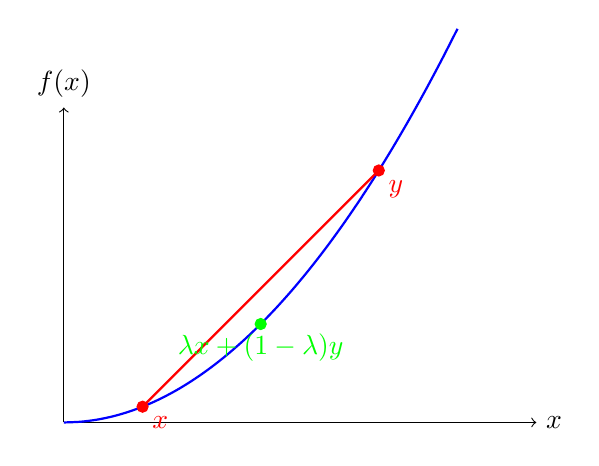
\begin{tikzpicture}
    \draw[->] (0,0) -- (6,0) node[right] {$x$};
    \draw[->] (0,0) -- (0,4) node[above] {$f(x)$};
    
    % Convex function
    \draw[blue, thick, domain=0:5, smooth, variable=\x] plot ({\x}, {0.2*\x*\x});
    
    % Two points
    \filldraw[red] (1,0.2) circle (2pt) node[below right] {$x$};
    \filldraw[red] (4,3.2) circle (2pt) node[below right] {$y$};
    
    % Line segment
    \draw[red, thick] (1,0.2) -- (4,3.2);
    
    % Midpoint
    \filldraw[green] (2.5,1.25) circle (2pt) node[below] {$\lambda x + (1-\lambda)y$};
    
    \end{tikzpicture}
    \caption{Example of a Convex Function}
    \label{fig:convex_function}
\end{figure}

\subsubsection{Convex Set}
A convex set means that the line segment connecting any two points in the set lies entirely within the set:
\begin{equation}
\lambda x + (1-\lambda)y \in S, \quad \forall x,y \in S, \forall \lambda \in [0,1]
\end{equation}

\begin{figure}[H]
    \centering
    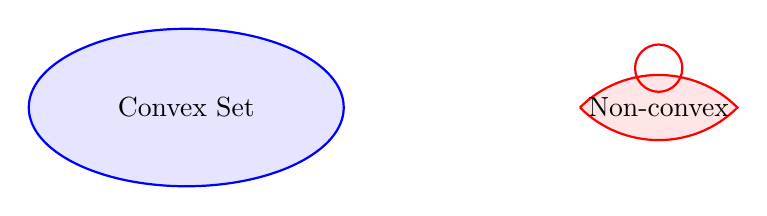
\begin{tikzpicture}
    % Convex set
    \draw[blue, thick, fill=blue!10] (0,0) ellipse (2 and 1);
    \node at (0,0) {Convex Set};
    
    % Non-convex set
    \draw[red, thick, fill=red!10] (5,0) to[out=45,in=135] (7,0) to[out=-135,in=-45] (5,0);
    \draw[red, thick] (6,0.5) circle (0.3);
    \node at (6,0) {Non-convex};
    \end{tikzpicture}
    \caption{Examples of Convex and Non-convex Sets}
    \label{fig:convex_nonconvex_sets}
\end{figure}

\subsubsection{Advantages of Convex Optimization}
Convex optimization holds special importance in optimization theory\sidenote{Effective algorithms and mathematical guarantees developed for convex optimization problems make solving these types of problems more reliable. The optimization problems within deep learning algorithms we frequently hear about today are generally convex optimization problems. The optimization algorithms used here are usually gradient descent methods. While they are very effective methods, they are generally inefficient in structural optimization problems.}:

\begin{itemize}
    \item \textbf{Local Optimum = Global Optimum:} A local minimum of a convex function is also the global minimum. This significantly simplifies the optimization process.
    \item \textbf{Stable Solution:} Regardless of the starting point, appropriate gradient-based algorithms converge to the same optimum point.
    \item \textbf{Efficient Algorithms:} Algorithms such as interior point methods and gradient descent can reach solutions in polynomial time for convex problems.
\end{itemize}

\begin{tcolorbox}[title=Example of Convex Optimization]
Quadratic programming problem:
\begin{equation}
\begin{aligned}
\min_{x \in \mathbb{R}^n} & \quad \frac{1}{2}x^TQx + c^Tx \\
\text{s.t.} & \quad Ax \leq b
\end{aligned}
\end{equation}

If $Q$ is a positive semi-definite matrix, this problem is convex and can be solved with efficient interior point methods.
\end{tcolorbox}

\subsubsection{Difficulties of Non-convex Optimization}
Non-convex optimization problems are frequently encountered challenges in structural optimization\sidenote{Most structural optimization problems are non-convex problems that can contain multiple local optima. This creates difficulties in finding the global optimum.}:

\begin{itemize}
    \item \textbf{Multiple Local Optima:} The function can contain multiple local minima, making it difficult to find the global optimum.
    \item \textbf{Starting Point Dependency:} Gradient-based algorithms can converge to different local optima depending on the starting point.
    \item \textbf{Computational Cost:} Generally, more comprehensive search methods are required to guarantee finding the global optimum, which increases computational cost.
\end{itemize}

\begin{tcolorbox}[title=Approaches to Non-convex Problems]
\begin{itemize}
    \item \textbf{Multiple Starting Points:} Multiple local optimizations are run from different starting points, and the best result is selected.
    \item \textbf{Metaheuristic Algorithms:} Methods such as genetic algorithms and particle swarm optimization try to approach the global optimum by exploring a wide solution space.
    \item \textbf{Convex Approximations:} The problem can be decomposed into convex sub-problems or solved using convex approximations (such as Sequential Convex Programming).
\end{itemize}
\end{tcolorbox}

\subsection{Constrained and Unconstrained Optimization}

\subsubsection{Unconstrained Optimization}
Unconstrained optimization, as the name suggests, refers to problems that do not contain any constraints, only requiring the minimization or maximization of the objective function. Mathematically:
\begin{equation}
\min_{x \in \mathbb{R}^n} f(x)
\end{equation}

\sidenote{Although unconstrained optimization is theoretically called "unconstrained," most engineering problems in practice contain physical or mathematical constraints in some way. The term "unconstrained" here means that there are no explicit constraints in the problem formulation.}

The main methods used to solve unconstrained optimization problems \sidenote{The principles of these five methods can be tested with Python code through the link:

\qrcode[height=1in]{https://github.com/btayfur/structural-optimization/blob/main/Code/Examples/Exmp2/}}:

\begin{itemize}
    \item \textbf{Gradient Descent Method:} Aims to reach the minimum by proceeding step by step in the direction of fastest decrease of the function (negative gradient direction). This method is widely used, especially in deep learning and machine learning applications.
    
    \item \textbf{Newton's Method:} Makes more intelligent decisions about both direction and step size by also using the function's second derivative (Hessian) information. Due to its quadratic convergence property, it converges faster than gradient descent under the right conditions.
    
    \item \textbf{Quasi-Newton Methods:} Methods that estimate the Hessian matrix approximately instead of calculating it directly to reduce the computational cost of Newton's method. BFGS and L-BFGS are among the most popular Quasi-Newton algorithms.
    
    \item \textbf{Conjugate Gradient Method:} A method that is particularly effective in large-scale problems and ensures that successive search directions are "conjugate" to each other.
    
    \item \textbf{Trust Region Methods:} Methods that determine a "trust region" in each iteration where the function can be locally well-modeled and search for the optimum within this region.
\end{itemize}

\begin{tcolorbox}[title=Mountain Climbing Analogy]
Let's think of a mountain climbing analogy to understand unconstrained optimization methods (for a maximization problem):

\begin{itemize}
    \item \textbf{Gradient Ascent:} You proceed in the steepest uphill direction at each step. Easy to implement but can progress slowly by zigzagging in narrow valleys.
    
    \item \textbf{Newton's Method:} You look not only at the slope of the ground (gradient) but also at the shape of the terrain (Hessian). This allows you to take large steps on flat areas and small, careful steps on steep slopes.
    
    \item \textbf{Quasi-Newton:} Instead of fully measuring the shape of the terrain, you estimate it from your previous steps. While not as effective as Newton, it requires much less effort.
\end{itemize}
\end{tcolorbox}

\subsubsection{Constrained Optimization}
Constrained optimization is much more common in modeling real-world problems and includes a set of constraints in addition to the objective function. These constraints represent the conditions that the solution must satisfy. Mathematical formulation:
\begin{equation}
\begin{aligned}
\min_{x \in \mathbb{R}^n} & \quad f(x) \\
\text{s.t.} & \quad g_i(x) \leq 0, \quad i = 1,\ldots,m \\
& \quad h_j(x) = 0, \quad j = 1,\ldots,p
\end{aligned}
\end{equation}

Here, $g_i(x) \leq 0$ represents inequality constraints, and $h_j(x) = 0$ represents equality constraints.

\sidenote{Structural optimization problems are almost always constrained problems. When you want to minimize the weight of a bridge, there are various constraints such as the bridge being able to carry certain loads, having a certain safety factor, and being constructible. An optimization without these constraints would not find practical application.}

The main methods used to solve constrained optimization problems:

\begin{itemize}
    \item \textbf{Lagrange Multipliers Method:} Defines additional variables called Lagrange multipliers for equality-constrained problems, transforming the constrained problem into an extended unconstrained problem. This method is particularly useful when constraints must be exactly satisfied.
    
    \item \textbf{Karush-Kuhn-Tucker (KKT) Conditions:} Optimality conditions valid for both equality and inequality constraints. KKT conditions are a generalization of the Lagrange multipliers method to inequality constraints.
    
    \item \textbf{Penalty Function Methods:} Transforms the constrained problem into an unconstrained problem by penalizing constraint violations. There are two main approaches:
    \begin{itemize}
        \item \textbf{Exterior Penalty Method:} Adds penalties for constraint violations, allows infeasible solutions but penalizes them.
        \item \textbf{Interior Penalty (Barrier) Method:} Adds an increasing penalty as the boundary of the feasible region is approached, ensuring the solution stays within the feasible region.
    \end{itemize}
    
    \item \textbf{Active Set Methods:} In each iteration, determines which constraints are believed to be active and solves a smaller subproblem. This is particularly effective in linear and quadratic programming problems.
    
    \item \textbf{Interior Point Methods:} Approaches the optimum while staying within the feasible region. Uses barrier functions but handles constraints directly. Very effective in large-scale linear and convex programming problems.
    
    \item \textbf{Sequential Quadratic Programming (SQP):} Solves constrained nonlinear problems by transforming them into a series of quadratic subproblems. Widely used in structural optimization.
\end{itemize}

\begin{tcolorbox}[title=Constrained Optimization Analogy: Path Finding]
You can think of constrained optimization as a path-finding problem where you have to follow certain rules while trying to find the best way to your destination:

\begin{itemize}
    \item \textbf{Your Goal (Objective Function):} To reach the mountain summit.
    \item \textbf{Your Constraints:} You can only walk on marked trails (equality constraints), you must stay away from certain dangerous areas (inequality constraints).
    
    \item \textbf{Lagrange Method:} Similar to continuously checking the trail map and dangerous areas while progressing.
    
    \item \textbf{Penalty Method:} If you leave the marked trail, you experience extra difficulty (getting stuck in mud, passing through thorny bushes, etc.). Despite these penalties, sometimes taking shortcuts can be advantageous.
    
    \item \textbf{Barrier Method:} You behave as if there's an invisible "repulsive force" around dangerous areas, retreating as you get closer. This way, you always stay in the safe region.
\end{itemize}
\end{tcolorbox}

\begin{tcolorbox}[title=Handling Constraints]
Methods to transform a constrained problem into an unconstrained problem:

\begin{itemize}
    \item \textbf{Exterior Penalty Method:} 
    \begin{equation}
    \min f(x) + c\sum\max(0,g_i(x))^2 + c\sum(h_j(x))^2
    \end{equation}
    
    Here $c > 0$ is the penalty parameter and is generally increased during iterations. As constraint violations increase, the penalty also increases, thus directing the algorithm toward the feasible region over time.
    
    \item \textbf{Interior Penalty (Barrier) Method:} 
    \begin{equation}
    \min f(x) - c\sum\ln(-g_i(x))
    \end{equation}
    
    This method is only defined when $g_i(x) < 0$ (i.e., within the feasible region) and as the constraint boundary is approached, $\ln(-g_i(x)) \to -\infty$, ensuring the solution stays within the feasible region. The $c$ parameter is generally decreased during iterations.
    
    \item \textbf{Augmented Lagrangian Method:} 
    \begin{equation}
    \min f(x) + \sum\lambda_j h_j(x) + \frac{c}{2}\sum(h_j(x))^2 + \sum\mu_i\max(0,g_i(x)) + \frac{c}{2}\sum\max(0,g_i(x))^2
    \end{equation}
    
    This method combines the advantages of Lagrange multipliers and penalty methods. Lagrange multipliers $\lambda_j$ and $\mu_i$ are updated in each iteration.
\end{itemize}
\end{tcolorbox}

\subsubsection{Comparison of Constrained and Unconstrained Optimization}

\begin{itemize}
    \item \textbf{Problem Difficulty:} Constrained problems are generally more difficult and require more specialized solution methods.
    
    \item \textbf{Solution Space:} In unconstrained problems, the entire search space can be used, while in constrained problems, the search is limited to the "feasible region."
    
    \item \textbf{Realism:} Real engineering problems are almost always constrained because designs must meet certain requirements.
    
    \item \textbf{Solution Strategy:} In solving constrained problems, the goal is generally to first satisfy the constraints, then optimize the objective function, or to handle these two goals in a balanced way.
\end{itemize}

\sidenote{Structural optimization problems generally contain quite complex constraints. For example, in the design of a skyscraper, while minimizing cost, many factors such as structural strength, user comfort, seismic performance, and wind loads must be considered as constraints. The nonlinearity of these constraints and their interaction with each other requires the development of special techniques to solve the problem.}

\subsection{Classification of Optimization Approaches}

\subsubsection{By Problem Structure}
Optimization problems can be categorized according to their mathematical structure, and this classification helps us determine which solution methods are appropriate:

\begin{itemize}
    \item \textbf{Linear Programming (LP)}
        \begin{itemize}
            \item Linear objective function: $f(x) = c^T x$
            \item Linear constraints: $Ax \leq b$, $Aeq \cdot x = beq$
            \item Basic solution methods: Simplex algorithm, Interior point methods
            \item Properties: Single global optimum, convex feasible region defined by constraints
            \item Application areas: Resource allocation, production planning, logistics optimization
        \end{itemize}
        
    \item \textbf{Nonlinear Programming (NLP)}
        \begin{itemize}
            \item Nonlinear objective function and/or constraints
            \item Subcategory - Convex Programming: Convex objective function, convex constraint set
            \item Subcategory - Non-convex Programming: Objective function and/or constraint set not convex
            \item Solution methods: Gradient-based methods (SQP, Interior point, BFGS), metaheuristic methods
            \item Application areas: Structural design, mechanical systems optimization, economic models
        \end{itemize}
        
    \item \textbf{Integer Programming (IP)}
        \begin{itemize}
            \item All variables must be integer: $x \in \mathbb{Z}^n$
            \item Subcategory - Mixed Integer Programming (MIP): Some variables integer, some continuous
            \item Subcategory - 0-1 Integer Programming: Variables can only take values 0 or 1
            \item Solution methods: Branch-and-bound, Cutting plane, Branch-and-cut
            \item Application areas: Scheduling problems, cutting/packing problems, topology optimization
        \end{itemize}
        
    \item \textbf{Stochastic Programming}
        \begin{itemize}
            \item Problems containing random variables
            \item Cases where uncertainty is modeled with probability distributions
            \item Solution methods: Scenario approach, sample average approximation, robust optimization
            \item Application areas: Risk management, portfolio optimization, structural design under uncertainty
        \end{itemize}
        
    \item \textbf{Multi-objective Programming}
        \begin{itemize}
            \item Simultaneous optimization of multiple objective functions
            \item Solution concept: Pareto-optimal solution set
            \item Solution methods: Weighted sum method, epsilon-constraint method, evolutionary algorithms like NSGA-II
            \item Application areas: Engineering design, environmental management, economic models
        \end{itemize}
\end{itemize}

\sidenote{A structural optimization problem generally carries characteristics of several of the above categories. For example, in a bridge design, section dimensions might be continuous variables while element types to be used might be integer variables. Additionally, material behavior might be expressed with nonlinear equations, and it might be necessary to optimize multiple criteria such as both cost and displacement. In this case, the problem becomes a mixed integer, nonlinear, multi-objective optimization problem.}

\subsubsection{By Solution Strategy}
Algorithms used to solve optimization problems can be categorized according to their search strategies:

\begin{itemize}
    \item \textbf{Deterministic Methods}
        \begin{itemize}
            \item \textbf{Gradient-based methods:} Progress in the direction of fastest improvement using derivative information of the function.
                \begin{itemize}
                    \item Advantages: Usually fast convergence, guaranteed reach to local optimum
                    \item Disadvantages: Getting stuck in local optima, derivative calculation requirement
                    \item Examples: Gradient descent, Newton, BFGS, Conjugate gradient
                \end{itemize}
                
            \item \textbf{Direct search methods:} Progress using function evaluations without derivative information.
                \begin{itemize}
                    \item Advantages: No derivatives required, suitable for noisy functions
                    \item Disadvantages: Usually slower convergence
                    \item Examples: Nelder-Mead simplex, Hooke-Jeeves pattern search
                \end{itemize}
                
            \item \textbf{Interior point methods:} Reach the optimum while staying within the feasible region.
                \begin{itemize}
                    \item Advantages: Effective in large-scale problems, polynomial time algorithm
                    \item Disadvantages: Complex implementation, starting point requirement
                    \item Examples: Primal-dual interior point, barrier methods
                \end{itemize}
        \end{itemize}
    
    \item \textbf{Stochastic/Metaheuristic Methods}
        \begin{itemize}
            \item \textbf{Evolutionary algorithms:} Mimic natural selection and genetic mechanisms.
                \begin{itemize}
                    \item Advantages: Potential to find global optimum, no derivatives required, suitable for parallel processing
                    \item Disadvantages: High computational cost, sensitive parameter tuning
                    \item Examples: Genetic algorithms, differential evolution, evolution strategies
                \end{itemize}
                
            \item \textbf{Swarm-based algorithms:} Search for solutions by modeling collective behaviors of animal groups.
                \begin{itemize}
                    \item Advantages: Easy implementation, effective in non-convex problems
                    \item Disadvantages: Weak theoretical guarantees, variable solution quality
                    \item Examples: Particle swarm optimization, ant colony optimization, bee algorithm
                \end{itemize}
                
            \item \textbf{Physics-based algorithms:} Perform optimization by mimicking physical processes.
                \begin{itemize}
                    \item Advantages: Ability to escape local optima
                    \item Disadvantages: Slow convergence, parameter sensitivity
                    \item Examples: Simulated annealing, harmony search, big bang-big crunch
                \end{itemize}
        \end{itemize}
    
    \item \textbf{Hybrid Methods} \sidenote{Hybrid methods combine the advantages of different approaches to provide more robust and effective solutions. For example, starting with a genetic algorithm for global search and then refining promising regions with a local gradient-based algorithm both increases the chance of finding the global optimum and ensures reaching a precise solution.}
        \begin{itemize}
            \item \textbf{Deterministic + Stochastic hybrid:} Combines advantages of both approaches.
                \begin{itemize}
                    \item Advantages: Combining global search with local optimization
                    \item Disadvantages: Complex implementation, difficult parameter tuning
                    \item Examples: Memetic algorithms, multi-start gradient methods
                \end{itemize}
                
            \item \textbf{Multi-level approaches:} Handles the problem at different detail levels.
                \begin{itemize}
                    \item Advantages: Ability to solve large and complex problems
                    \item Disadvantages: Problem-specific design requirement
                    \item Examples: Coarse-fine grid methods, hierarchical optimization
                \end{itemize}
                
            \item \textbf{Adaptive strategies:} Changes algorithm parameters or strategies during the optimization process.
                \begin{itemize}
                    \item Advantages: Dynamic adaptation to problem characteristics
                    \item Disadvantages: Complex control mechanisms
                    \item Examples: Adaptive metaheuristic methods, self-adaptive evolution strategies \sidenote{In structural optimization problems, since the computational cost of finite element analysis is generally high, algorithms that perform as few function evaluations as possible are preferred. Therefore, surrogate model-based optimization methods are becoming increasingly popular. These methods speed up the optimization process by using approximate models that can be calculated faster instead of real analysis.} 
                \end{itemize}
        \end{itemize}
\end{itemize}

\begin{tcolorbox}[title=Optimization Algorithm Selection]
Which algorithm is most suitable for an optimization problem depends on the problem's characteristics:

\begin{itemize}
    \item \textbf{Problem size:} Interior point methods, gradient-based methods, or specially designed metaheuristic methods are suitable for large-scale problems.
    
    \item \textbf{Derivative information:} If derivative calculation is possible and economical, gradient-based methods are generally faster. If derivative calculation is difficult or impossible, direct search or metaheuristic methods are preferred.
    
    \item \textbf{Problem nature:} Deterministic methods are generally sufficient for convex problems. Metaheuristic or hybrid methods are more suitable for non-convex, multimodal problems.
    
    \item \textbf{Computational budget:} If computational resources are limited, more efficient deterministic methods may be preferred. If high computational power is available, more comprehensive global search methods can be used.
    
    \item \textbf{Importance of feasible solution:} If feasible solutions are needed in intermediate iterations, methods that stay within the feasible region (interior point, barrier methods) may be preferred.
\end{itemize}
\end{tcolorbox} 